% vim:spell spelllang=sk
\subsection{Analýza RLC obvodov}

RLC analýza je analýza obvodov zložených z odporov, kondenzátorov a
cievok. Tieto rezonančné obvody hrajú dôležitú úlohu vo fyzike.
Základným krokom, ktorý nám umožní ich analýzu pomocou Fourierovej
transformácie je princíp superpozície
\begin{veta}[Princíp superpozície]
 Nech $U_1(t), I_1(t)$ a $U_2(t), I_2(t)$ sú dve riešenia RLC obvodu
 \footnote{Pod pojmom riešenie myslíme "riešenie sústavy
 diferenciálnych rovníc popísaných daným obvodom"}.
 Potom $U(t)=a_1 U_1(t) + a_2 U_2(t), I(t)=a_1 I_1(t) + a_2 I_2(t)$ je
 tiež riešením daného obvodu
\end{veta}
\begin{dokaz}
    Načrtneme si základné črty dôkazu, nepôjdeme však do podrobností.
    Každý RLC obvod vieme popísať ako sústavu diferenciálnych rovníc - 
    jedna rovnica pre vzťah napätia a prúdu na každej súčiastke +
    rovnice pre všetky uzly, ktoré popisujú nemožnosť hromadenia sa
    náboja na jednom mieste.
    Rovnice pre jednotlivé súčiastky
    \begin{itemize}
        \item Rezistor: $U(t) = R I(t)$
        \item Kondenzátor: $I(t) = C \pd{U}{t}$
        \item Cievka: $U(t) = L \pd{I}{t}$
        \item Uzol: $\sum_{k} I_k(t) = 0$
    \end{itemize}
    Všetky tieto 4 typy diferenciálnych rovníc majú spoločnú vlastnosť
    - linearitu medzi napätím a prúdom. Nie je tažké overiť, že pre ne
      platí princíp superpozície. Potom ale platí princíp superpozície
      pre celú sústavu týchto rovníc a teda pre RLC obvod.
\end{dokaz}
\begin{poznamka}
    Čitateľ mohol nadubodnúť dojem, že superpozícia u obvodov je
    evidentná. Veľmi rýchlo ho ale vyvedieme z omylu. Už len taká
    jednoduchá súčiastka ako dióda je prudko nelineárna. Ideálna dióda
    prepúšťa prúd len jedným smerom. Aplikáciou princípu superpozície
    dvoch prúdov rovnakej veľkosti ale opačného smeru by sme ľakho
    mohli dospieť k záveru, že za nulového prúdu tečúceho obvodom
    tečie nenulový prúd diódou. Zjavný spor. Superpozícia preto nie je 
    \todo{allmighty} nástroj na riešenie všetkých elektrických obvodov
\end{poznamka}

Aby sme mohli ďalej pokračovať, musíme najskôr vyriešiť rovnice pre
jednotlivé súčiastky, čo nám dá predstavu o súvislosti napätia a
prúdu. Riešenie pre odpory je triviálne, nakoľko ak $I(t)=f(t)$, potom
$U(t)=R f(t)$. Zaujímavejší je ale kondenzátor a cievka
\begin{lema}[Jedno riešenie pre kondenzátor]
    Nech $U(t) = \sin (\omega t)$ a nech $I(t) = C\omega \cos (\omega t)$.
    Potom $U,I$ je riešením rovnice pre kondenzátor.
\end{lema}
Môžeme si všimnúť zaujímavú vec - prúd "zaostáva" za napätím o pol
periódy. V prípade cievky to bude presne opačne, ako sa môžeme
presvedčiť v nasledujúcej leme:
\begin{lema}[Jedno riešenie pre cievku]
 Nech $U(t) = \cos (\omega t)$ a $I(t) = \frac{1}{L \omega} \sin (\omega t)$.
 Potom $U,I$ je riešením rovnice pre cievku
\end{lema}

Riešenia pre odpor, kondenzátor a cievku nám dávajú jasné pozorovanie
- ak je napätie na súčiastke sínusoidné, prúd má tiež tvar sínusoidy,
  ale posunutej. Preto je prirodzené zaviesť nasledujúce rozšírenie.

\begin{definicia}[Komplexný prúd, napätie]
    Nech má napätie alebo prúd priebeh $U(t) = U_0 \cos(\omega t +
    \phi)$. Označme
    $\mathcal{U} = U_0 e^{\imag \omega t + \phi}$ a nazvime ho komplexným
    napätím. Potom platí $U(t) = \Re \mathcal{U}(t)$. V ďalšom texte
    budeme kvôli pohodlnosti 
    skrývať fázový posun $\phi$ do komplexnej konštanty $U_0$.
    Podobne, komplexný prúd označíme ako $\mathcal{I}$.
\end{definicia}

Využitím komplexného napätia a prúdu vieme rovnice pre tieto tri
súčiastky zhrnúť do rovnice
\begin{equation}
    \mathcal{U} = \mathcal{I} Z
\end{equation}
Kde komplexná veličina $Z$ sa nazýva impedancia a platí pre ňu
\begin{itemize}
   \item $Z=R$ pre odpor
   \item $Z=\frac{1}{\imag C \omega}$ pre kondenzátor
   \item $Z=\imag L \omega$ pre cievku
\end{itemize}

Fourierova analýza nám pomôže previesť ľubovoľný signál práve na tieto
harmonické zložky, kde vieme obvod jednoducho vyriešiť a poskladať
naspäť pomocou princípu superpozície. Tieto myšlienky si ukážeme na
periodickom nabíjaní a vybíjaní kondenzátora.

Uvažujme jednoduchý RC obvod na obrázku \ref{fig:rc_obvod}

\begin{figure}[htp]
    \centering
    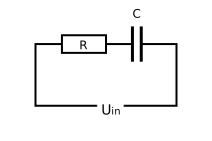
\includegraphics{obrazky/fyzika/rlc/rc_obvod}
    \caption{Jednoduchý RC obvod}
    \label{fig:rc_obvod}
\end{figure}

Ide o sériový obvod. Napätie na kondenzátore môžeme vypočítať
ako
\begin{equation}
    \mathcal{U}_C = \mathcal{U}_{in} \frac{Z_C}{Z_C+Z_R} =
            \mathcal{U}_{in} \frac{\frac{1}{\imag C \omega}}{
                R + \frac{1}{\imag C \omega}} = 
                \mathcal{U}_{in} \frac{1}{1 + \imag \omega RC}
    \label{eq:rc_u_kondenzator}
\end{equation}
Zaujímala by nás odozva na pílový signál prezentovaný v príklade
\todo{ref}. Ako sme už niekoľko krát použili, Fourierov rad daného
signálu je (\todo{ref})
\begin{equation}
    f(x) = \frac{1}{2} + \frac{2}{\pi} 
        \sum_{m=1}^{\infty} \frac{\sin((2m-1)x}{2m-1}
\end{equation}
Nám bude viacej vyhovovať komplexný tvar, ktorý dostaneme vyžitím
rovnice \ref{eq:koeficienty_to_exp}.
\begin{align}
    f(x) &= \sum_{m=-\infty}^{\infty} c_m e^{\imag m x} \\
    c_0 &= \frac{1}{2} \\
    c_m &= \imag \frac{1}{\pi} \frac{1}{m}, \quad m\in \Z 
        \text{je nepárne}
\end{align}
Budeme pokračovať ďalej, ale ešte predtým vyriešime 2 problémy:
Prvým je
$\omega=0$. Vtedy je totiž impedancia kondenzátora podľa vzorca
nekonečná a odvodenie \ref{eq:rc_u_kondenzator} nemusí byť korektné.
V tomto prípade ale ide o voľný obvod, ktorým netečie žiadnu prúd a
napätie $\mathcal{U}_C = \mathcal{U}_{in}$.

Druhým problémom je $\omega<0$. Môžeme sa ale ľahko presvedčiť, že
toto je iba problém interpretácie (ako sa dá interpretovať záporná
uhlová rýchlosť resp. frekvencia?). Matematická stránka veci ostáva
perfektne korektná.

Podľa princípu superpozície teda môžeme písať
\begin{align}
    \mathcal{U}_C(t) = \frac{1}{2} +
        \frac{1}{\pi} \sum_{m=0}^{\infty}
            \imag \frac{1}{2m+1} \left(
                \frac{e^{\imag (2m+1) t} }{1 + \imag (2m+1) RC} -
                \frac{e^{- \imag (2m+1) t} }{1 - \imag (2m+1) RC}
            \right)
\end{align}
\begin{poznamka}
    Môžeme si všimnúť, že princíp superpozície v tejto forme je
    vlastne inverzná Fourierova transformácia
\end{poznamka}
Upravovaním výrazu v zátvorke dostávame
\begin{equation}
    \begin{split}
    \frac{e^{\imag \omega t}}{1 + \imag \omega RC} -
    \frac{e^{- \imag \omega t}}{1 - \imag \omega RC}  &= 
    \frac{ (1-\imag \omega RC) e^{\imag \omega t} -
           (1-\imag \omega RC) e^{\imag \omega t} +
    }{1 + \omega^2 R^2 C^2} \\&=
    \frac{2 \imag \sin (\omega t) - 2 \imag \omega RC \cos(\omega t)}{1 + \omega^2 R^2 C^2}
    \end{split}
\end{equation}

Spätným dosadením do \todo{ref} máme

\begin{align}
    \mathcal{U}_C(t) = \frac{1}{2} +
        \frac{2}{\pi} \sum_{m=0}^{\infty} \frac{1}{2m+1}
         \frac{\sin ((2m+1) t) - (2m+1) RC \cos((2m+1)t)}
         {1+(2m+1)^2 R^2 C^2}
\end{align}
Na obrázku \ref{fig:rc_priebeh} môžeme vidieť 100-té čiastočné súčty
tejto postupnosti. Na porovnanie sme ku grafom spe pripojili graf funkcie
$e^{-t/RC}$ s posunutím začiatkom, čo je klasický výsledok riešenie
diferenciálnej rovnice pre tento obvod. Môžeme si všimnúť, že pokiaľ
je dĺžka pulzu dostatočne dlhá oproti exponenciále, naše riešenie je
správne. V skutočnosti, exponenciálu by sme dostali ako výsledok
našeho výpočtu s Fourierovou transformáciou funkcie 
$\frac{1}{2} (1+\sgn x)$.

\begin{figure}[htp]
    \centering
    \includegraphics{obrazky/fyzika/rlc/rc_priebeh_01}
    \includegraphics{obrazky/fyzika/rlc/rc_priebeh_05}
    \includegraphics{obrazky/fyzika/rlc/rc_priebeh_10}
    \includegraphics{obrazky/fyzika/rlc/rc_priebeh_20}
    \caption{Priebeh napätia postupne pre $RC=0.1,0.5,1,2$}
    \label{fig:rc_priebeh}
\end{figure}

\todo{lit:rlc-difeq}
\todo{lit:wiki:complex-impedance}
\todo{lit:circuit-analysis}
